
% Default to the notebook output style

    


% Inherit from the specified cell style.




    
\documentclass[11pt]{article}

    
    
    \usepackage[T1]{fontenc}
    % Nicer default font (+ math font) than Computer Modern for most use cases
    \usepackage{mathpazo}

    % Basic figure setup, for now with no caption control since it's done
    % automatically by Pandoc (which extracts ![](path) syntax from Markdown).
    \usepackage{graphicx}
    % We will generate all images so they have a width \maxwidth. This means
    % that they will get their normal width if they fit onto the page, but
    % are scaled down if they would overflow the margins.
    \makeatletter
    \def\maxwidth{\ifdim\Gin@nat@width>\linewidth\linewidth
    \else\Gin@nat@width\fi}
    \makeatother
    \let\Oldincludegraphics\includegraphics
    % Set max figure width to be 80% of text width, for now hardcoded.
    \renewcommand{\includegraphics}[1]{\Oldincludegraphics[width=.8\maxwidth]{#1}}
    % Ensure that by default, figures have no caption (until we provide a
    % proper Figure object with a Caption API and a way to capture that
    % in the conversion process - todo).
    \usepackage{caption}
    \DeclareCaptionLabelFormat{nolabel}{}
    \captionsetup{labelformat=nolabel}

    \usepackage{adjustbox} % Used to constrain images to a maximum size 
    \usepackage{xcolor} % Allow colors to be defined
    \usepackage{enumerate} % Needed for markdown enumerations to work
    \usepackage{geometry} % Used to adjust the document margins
    \usepackage{amsmath} % Equations
    \usepackage{amssymb} % Equations
    \usepackage{textcomp} % defines textquotesingle
    % Hack from http://tex.stackexchange.com/a/47451/13684:
    \AtBeginDocument{%
        \def\PYZsq{\textquotesingle}% Upright quotes in Pygmentized code
    }
    \usepackage{upquote} % Upright quotes for verbatim code
    \usepackage{eurosym} % defines \euro
    \usepackage[mathletters]{ucs} % Extended unicode (utf-8) support
    \usepackage[utf8x]{inputenc} % Allow utf-8 characters in the tex document
    \usepackage{fancyvrb} % verbatim replacement that allows latex
    \usepackage{grffile} % extends the file name processing of package graphics 
                         % to support a larger range 
    % The hyperref package gives us a pdf with properly built
    % internal navigation ('pdf bookmarks' for the table of contents,
    % internal cross-reference links, web links for URLs, etc.)
    \usepackage{hyperref}
    \usepackage{longtable} % longtable support required by pandoc >1.10
    \usepackage{booktabs}  % table support for pandoc > 1.12.2
    \usepackage[inline]{enumitem} % IRkernel/repr support (it uses the enumerate* environment)
    \usepackage[normalem]{ulem} % ulem is needed to support strikethroughs (\sout)
                                % normalem makes italics be italics, not underlines
    

    
    
    % Colors for the hyperref package
    \definecolor{urlcolor}{rgb}{0,.145,.698}
    \definecolor{linkcolor}{rgb}{.71,0.21,0.01}
    \definecolor{citecolor}{rgb}{.12,.54,.11}

    % ANSI colors
    \definecolor{ansi-black}{HTML}{3E424D}
    \definecolor{ansi-black-intense}{HTML}{282C36}
    \definecolor{ansi-red}{HTML}{E75C58}
    \definecolor{ansi-red-intense}{HTML}{B22B31}
    \definecolor{ansi-green}{HTML}{00A250}
    \definecolor{ansi-green-intense}{HTML}{007427}
    \definecolor{ansi-yellow}{HTML}{DDB62B}
    \definecolor{ansi-yellow-intense}{HTML}{B27D12}
    \definecolor{ansi-blue}{HTML}{208FFB}
    \definecolor{ansi-blue-intense}{HTML}{0065CA}
    \definecolor{ansi-magenta}{HTML}{D160C4}
    \definecolor{ansi-magenta-intense}{HTML}{A03196}
    \definecolor{ansi-cyan}{HTML}{60C6C8}
    \definecolor{ansi-cyan-intense}{HTML}{258F8F}
    \definecolor{ansi-white}{HTML}{C5C1B4}
    \definecolor{ansi-white-intense}{HTML}{A1A6B2}

    % commands and environments needed by pandoc snippets
    % extracted from the output of `pandoc -s`
    \providecommand{\tightlist}{%
      \setlength{\itemsep}{0pt}\setlength{\parskip}{0pt}}
    \DefineVerbatimEnvironment{Highlighting}{Verbatim}{commandchars=\\\{\}}
    % Add ',fontsize=\small' for more characters per line
    \newenvironment{Shaded}{}{}
    \newcommand{\KeywordTok}[1]{\textcolor[rgb]{0.00,0.44,0.13}{\textbf{{#1}}}}
    \newcommand{\DataTypeTok}[1]{\textcolor[rgb]{0.56,0.13,0.00}{{#1}}}
    \newcommand{\DecValTok}[1]{\textcolor[rgb]{0.25,0.63,0.44}{{#1}}}
    \newcommand{\BaseNTok}[1]{\textcolor[rgb]{0.25,0.63,0.44}{{#1}}}
    \newcommand{\FloatTok}[1]{\textcolor[rgb]{0.25,0.63,0.44}{{#1}}}
    \newcommand{\CharTok}[1]{\textcolor[rgb]{0.25,0.44,0.63}{{#1}}}
    \newcommand{\StringTok}[1]{\textcolor[rgb]{0.25,0.44,0.63}{{#1}}}
    \newcommand{\CommentTok}[1]{\textcolor[rgb]{0.38,0.63,0.69}{\textit{{#1}}}}
    \newcommand{\OtherTok}[1]{\textcolor[rgb]{0.00,0.44,0.13}{{#1}}}
    \newcommand{\AlertTok}[1]{\textcolor[rgb]{1.00,0.00,0.00}{\textbf{{#1}}}}
    \newcommand{\FunctionTok}[1]{\textcolor[rgb]{0.02,0.16,0.49}{{#1}}}
    \newcommand{\RegionMarkerTok}[1]{{#1}}
    \newcommand{\ErrorTok}[1]{\textcolor[rgb]{1.00,0.00,0.00}{\textbf{{#1}}}}
    \newcommand{\NormalTok}[1]{{#1}}
    
    % Additional commands for more recent versions of Pandoc
    \newcommand{\ConstantTok}[1]{\textcolor[rgb]{0.53,0.00,0.00}{{#1}}}
    \newcommand{\SpecialCharTok}[1]{\textcolor[rgb]{0.25,0.44,0.63}{{#1}}}
    \newcommand{\VerbatimStringTok}[1]{\textcolor[rgb]{0.25,0.44,0.63}{{#1}}}
    \newcommand{\SpecialStringTok}[1]{\textcolor[rgb]{0.73,0.40,0.53}{{#1}}}
    \newcommand{\ImportTok}[1]{{#1}}
    \newcommand{\DocumentationTok}[1]{\textcolor[rgb]{0.73,0.13,0.13}{\textit{{#1}}}}
    \newcommand{\AnnotationTok}[1]{\textcolor[rgb]{0.38,0.63,0.69}{\textbf{\textit{{#1}}}}}
    \newcommand{\CommentVarTok}[1]{\textcolor[rgb]{0.38,0.63,0.69}{\textbf{\textit{{#1}}}}}
    \newcommand{\VariableTok}[1]{\textcolor[rgb]{0.10,0.09,0.49}{{#1}}}
    \newcommand{\ControlFlowTok}[1]{\textcolor[rgb]{0.00,0.44,0.13}{\textbf{{#1}}}}
    \newcommand{\OperatorTok}[1]{\textcolor[rgb]{0.40,0.40,0.40}{{#1}}}
    \newcommand{\BuiltInTok}[1]{{#1}}
    \newcommand{\ExtensionTok}[1]{{#1}}
    \newcommand{\PreprocessorTok}[1]{\textcolor[rgb]{0.74,0.48,0.00}{{#1}}}
    \newcommand{\AttributeTok}[1]{\textcolor[rgb]{0.49,0.56,0.16}{{#1}}}
    \newcommand{\InformationTok}[1]{\textcolor[rgb]{0.38,0.63,0.69}{\textbf{\textit{{#1}}}}}
    \newcommand{\WarningTok}[1]{\textcolor[rgb]{0.38,0.63,0.69}{\textbf{\textit{{#1}}}}}
    
    
    % Define a nice break command that doesn't care if a line doesn't already
    % exist.
    \def\br{\hspace*{\fill} \\* }
    % Math Jax compatability definitions
    \def\gt{>}
    \def\lt{<}
    % Document parameters
    \title{pixelDenoising}
    
    
    

    % Pygments definitions
    
\makeatletter
\def\PY@reset{\let\PY@it=\relax \let\PY@bf=\relax%
    \let\PY@ul=\relax \let\PY@tc=\relax%
    \let\PY@bc=\relax \let\PY@ff=\relax}
\def\PY@tok#1{\csname PY@tok@#1\endcsname}
\def\PY@toks#1+{\ifx\relax#1\empty\else%
    \PY@tok{#1}\expandafter\PY@toks\fi}
\def\PY@do#1{\PY@bc{\PY@tc{\PY@ul{%
    \PY@it{\PY@bf{\PY@ff{#1}}}}}}}
\def\PY#1#2{\PY@reset\PY@toks#1+\relax+\PY@do{#2}}

\expandafter\def\csname PY@tok@w\endcsname{\def\PY@tc##1{\textcolor[rgb]{0.73,0.73,0.73}{##1}}}
\expandafter\def\csname PY@tok@c\endcsname{\let\PY@it=\textit\def\PY@tc##1{\textcolor[rgb]{0.25,0.50,0.50}{##1}}}
\expandafter\def\csname PY@tok@cp\endcsname{\def\PY@tc##1{\textcolor[rgb]{0.74,0.48,0.00}{##1}}}
\expandafter\def\csname PY@tok@k\endcsname{\let\PY@bf=\textbf\def\PY@tc##1{\textcolor[rgb]{0.00,0.50,0.00}{##1}}}
\expandafter\def\csname PY@tok@kp\endcsname{\def\PY@tc##1{\textcolor[rgb]{0.00,0.50,0.00}{##1}}}
\expandafter\def\csname PY@tok@kt\endcsname{\def\PY@tc##1{\textcolor[rgb]{0.69,0.00,0.25}{##1}}}
\expandafter\def\csname PY@tok@o\endcsname{\def\PY@tc##1{\textcolor[rgb]{0.40,0.40,0.40}{##1}}}
\expandafter\def\csname PY@tok@ow\endcsname{\let\PY@bf=\textbf\def\PY@tc##1{\textcolor[rgb]{0.67,0.13,1.00}{##1}}}
\expandafter\def\csname PY@tok@nb\endcsname{\def\PY@tc##1{\textcolor[rgb]{0.00,0.50,0.00}{##1}}}
\expandafter\def\csname PY@tok@nf\endcsname{\def\PY@tc##1{\textcolor[rgb]{0.00,0.00,1.00}{##1}}}
\expandafter\def\csname PY@tok@nc\endcsname{\let\PY@bf=\textbf\def\PY@tc##1{\textcolor[rgb]{0.00,0.00,1.00}{##1}}}
\expandafter\def\csname PY@tok@nn\endcsname{\let\PY@bf=\textbf\def\PY@tc##1{\textcolor[rgb]{0.00,0.00,1.00}{##1}}}
\expandafter\def\csname PY@tok@ne\endcsname{\let\PY@bf=\textbf\def\PY@tc##1{\textcolor[rgb]{0.82,0.25,0.23}{##1}}}
\expandafter\def\csname PY@tok@nv\endcsname{\def\PY@tc##1{\textcolor[rgb]{0.10,0.09,0.49}{##1}}}
\expandafter\def\csname PY@tok@no\endcsname{\def\PY@tc##1{\textcolor[rgb]{0.53,0.00,0.00}{##1}}}
\expandafter\def\csname PY@tok@nl\endcsname{\def\PY@tc##1{\textcolor[rgb]{0.63,0.63,0.00}{##1}}}
\expandafter\def\csname PY@tok@ni\endcsname{\let\PY@bf=\textbf\def\PY@tc##1{\textcolor[rgb]{0.60,0.60,0.60}{##1}}}
\expandafter\def\csname PY@tok@na\endcsname{\def\PY@tc##1{\textcolor[rgb]{0.49,0.56,0.16}{##1}}}
\expandafter\def\csname PY@tok@nt\endcsname{\let\PY@bf=\textbf\def\PY@tc##1{\textcolor[rgb]{0.00,0.50,0.00}{##1}}}
\expandafter\def\csname PY@tok@nd\endcsname{\def\PY@tc##1{\textcolor[rgb]{0.67,0.13,1.00}{##1}}}
\expandafter\def\csname PY@tok@s\endcsname{\def\PY@tc##1{\textcolor[rgb]{0.73,0.13,0.13}{##1}}}
\expandafter\def\csname PY@tok@sd\endcsname{\let\PY@it=\textit\def\PY@tc##1{\textcolor[rgb]{0.73,0.13,0.13}{##1}}}
\expandafter\def\csname PY@tok@si\endcsname{\let\PY@bf=\textbf\def\PY@tc##1{\textcolor[rgb]{0.73,0.40,0.53}{##1}}}
\expandafter\def\csname PY@tok@se\endcsname{\let\PY@bf=\textbf\def\PY@tc##1{\textcolor[rgb]{0.73,0.40,0.13}{##1}}}
\expandafter\def\csname PY@tok@sr\endcsname{\def\PY@tc##1{\textcolor[rgb]{0.73,0.40,0.53}{##1}}}
\expandafter\def\csname PY@tok@ss\endcsname{\def\PY@tc##1{\textcolor[rgb]{0.10,0.09,0.49}{##1}}}
\expandafter\def\csname PY@tok@sx\endcsname{\def\PY@tc##1{\textcolor[rgb]{0.00,0.50,0.00}{##1}}}
\expandafter\def\csname PY@tok@m\endcsname{\def\PY@tc##1{\textcolor[rgb]{0.40,0.40,0.40}{##1}}}
\expandafter\def\csname PY@tok@gh\endcsname{\let\PY@bf=\textbf\def\PY@tc##1{\textcolor[rgb]{0.00,0.00,0.50}{##1}}}
\expandafter\def\csname PY@tok@gu\endcsname{\let\PY@bf=\textbf\def\PY@tc##1{\textcolor[rgb]{0.50,0.00,0.50}{##1}}}
\expandafter\def\csname PY@tok@gd\endcsname{\def\PY@tc##1{\textcolor[rgb]{0.63,0.00,0.00}{##1}}}
\expandafter\def\csname PY@tok@gi\endcsname{\def\PY@tc##1{\textcolor[rgb]{0.00,0.63,0.00}{##1}}}
\expandafter\def\csname PY@tok@gr\endcsname{\def\PY@tc##1{\textcolor[rgb]{1.00,0.00,0.00}{##1}}}
\expandafter\def\csname PY@tok@ge\endcsname{\let\PY@it=\textit}
\expandafter\def\csname PY@tok@gs\endcsname{\let\PY@bf=\textbf}
\expandafter\def\csname PY@tok@gp\endcsname{\let\PY@bf=\textbf\def\PY@tc##1{\textcolor[rgb]{0.00,0.00,0.50}{##1}}}
\expandafter\def\csname PY@tok@go\endcsname{\def\PY@tc##1{\textcolor[rgb]{0.53,0.53,0.53}{##1}}}
\expandafter\def\csname PY@tok@gt\endcsname{\def\PY@tc##1{\textcolor[rgb]{0.00,0.27,0.87}{##1}}}
\expandafter\def\csname PY@tok@err\endcsname{\def\PY@bc##1{\setlength{\fboxsep}{0pt}\fcolorbox[rgb]{1.00,0.00,0.00}{1,1,1}{\strut ##1}}}
\expandafter\def\csname PY@tok@kc\endcsname{\let\PY@bf=\textbf\def\PY@tc##1{\textcolor[rgb]{0.00,0.50,0.00}{##1}}}
\expandafter\def\csname PY@tok@kd\endcsname{\let\PY@bf=\textbf\def\PY@tc##1{\textcolor[rgb]{0.00,0.50,0.00}{##1}}}
\expandafter\def\csname PY@tok@kn\endcsname{\let\PY@bf=\textbf\def\PY@tc##1{\textcolor[rgb]{0.00,0.50,0.00}{##1}}}
\expandafter\def\csname PY@tok@kr\endcsname{\let\PY@bf=\textbf\def\PY@tc##1{\textcolor[rgb]{0.00,0.50,0.00}{##1}}}
\expandafter\def\csname PY@tok@bp\endcsname{\def\PY@tc##1{\textcolor[rgb]{0.00,0.50,0.00}{##1}}}
\expandafter\def\csname PY@tok@fm\endcsname{\def\PY@tc##1{\textcolor[rgb]{0.00,0.00,1.00}{##1}}}
\expandafter\def\csname PY@tok@vc\endcsname{\def\PY@tc##1{\textcolor[rgb]{0.10,0.09,0.49}{##1}}}
\expandafter\def\csname PY@tok@vg\endcsname{\def\PY@tc##1{\textcolor[rgb]{0.10,0.09,0.49}{##1}}}
\expandafter\def\csname PY@tok@vi\endcsname{\def\PY@tc##1{\textcolor[rgb]{0.10,0.09,0.49}{##1}}}
\expandafter\def\csname PY@tok@vm\endcsname{\def\PY@tc##1{\textcolor[rgb]{0.10,0.09,0.49}{##1}}}
\expandafter\def\csname PY@tok@sa\endcsname{\def\PY@tc##1{\textcolor[rgb]{0.73,0.13,0.13}{##1}}}
\expandafter\def\csname PY@tok@sb\endcsname{\def\PY@tc##1{\textcolor[rgb]{0.73,0.13,0.13}{##1}}}
\expandafter\def\csname PY@tok@sc\endcsname{\def\PY@tc##1{\textcolor[rgb]{0.73,0.13,0.13}{##1}}}
\expandafter\def\csname PY@tok@dl\endcsname{\def\PY@tc##1{\textcolor[rgb]{0.73,0.13,0.13}{##1}}}
\expandafter\def\csname PY@tok@s2\endcsname{\def\PY@tc##1{\textcolor[rgb]{0.73,0.13,0.13}{##1}}}
\expandafter\def\csname PY@tok@sh\endcsname{\def\PY@tc##1{\textcolor[rgb]{0.73,0.13,0.13}{##1}}}
\expandafter\def\csname PY@tok@s1\endcsname{\def\PY@tc##1{\textcolor[rgb]{0.73,0.13,0.13}{##1}}}
\expandafter\def\csname PY@tok@mb\endcsname{\def\PY@tc##1{\textcolor[rgb]{0.40,0.40,0.40}{##1}}}
\expandafter\def\csname PY@tok@mf\endcsname{\def\PY@tc##1{\textcolor[rgb]{0.40,0.40,0.40}{##1}}}
\expandafter\def\csname PY@tok@mh\endcsname{\def\PY@tc##1{\textcolor[rgb]{0.40,0.40,0.40}{##1}}}
\expandafter\def\csname PY@tok@mi\endcsname{\def\PY@tc##1{\textcolor[rgb]{0.40,0.40,0.40}{##1}}}
\expandafter\def\csname PY@tok@il\endcsname{\def\PY@tc##1{\textcolor[rgb]{0.40,0.40,0.40}{##1}}}
\expandafter\def\csname PY@tok@mo\endcsname{\def\PY@tc##1{\textcolor[rgb]{0.40,0.40,0.40}{##1}}}
\expandafter\def\csname PY@tok@ch\endcsname{\let\PY@it=\textit\def\PY@tc##1{\textcolor[rgb]{0.25,0.50,0.50}{##1}}}
\expandafter\def\csname PY@tok@cm\endcsname{\let\PY@it=\textit\def\PY@tc##1{\textcolor[rgb]{0.25,0.50,0.50}{##1}}}
\expandafter\def\csname PY@tok@cpf\endcsname{\let\PY@it=\textit\def\PY@tc##1{\textcolor[rgb]{0.25,0.50,0.50}{##1}}}
\expandafter\def\csname PY@tok@c1\endcsname{\let\PY@it=\textit\def\PY@tc##1{\textcolor[rgb]{0.25,0.50,0.50}{##1}}}
\expandafter\def\csname PY@tok@cs\endcsname{\let\PY@it=\textit\def\PY@tc##1{\textcolor[rgb]{0.25,0.50,0.50}{##1}}}

\def\PYZbs{\char`\\}
\def\PYZus{\char`\_}
\def\PYZob{\char`\{}
\def\PYZcb{\char`\}}
\def\PYZca{\char`\^}
\def\PYZam{\char`\&}
\def\PYZlt{\char`\<}
\def\PYZgt{\char`\>}
\def\PYZsh{\char`\#}
\def\PYZpc{\char`\%}
\def\PYZdl{\char`\$}
\def\PYZhy{\char`\-}
\def\PYZsq{\char`\'}
\def\PYZdq{\char`\"}
\def\PYZti{\char`\~}
% for compatibility with earlier versions
\def\PYZat{@}
\def\PYZlb{[}
\def\PYZrb{]}
\makeatother


    % Exact colors from NB
    \definecolor{incolor}{rgb}{0.0, 0.0, 0.5}
    \definecolor{outcolor}{rgb}{0.545, 0.0, 0.0}



    
    % Prevent overflowing lines due to hard-to-break entities
    \sloppy 
    % Setup hyperref package
    \hypersetup{
      breaklinks=true,  % so long urls are correctly broken across lines
      colorlinks=true,
      urlcolor=urlcolor,
      linkcolor=linkcolor,
      citecolor=citecolor,
      }
    % Slightly bigger margins than the latex defaults
    
    \geometry{verbose,tmargin=1in,bmargin=1in,lmargin=1in,rmargin=1in}
    
    

    \begin{document}
    
    
    \maketitle
    
    

    
    \section{README from code source}\label{readme-from-code-source}

\subsection{NCS}\label{ncs}

NCS is a Noise Correction Algorithm for sCMOS cameras.

\subsection{Abstract}\label{abstract}

Scientific CMOS (sCMOS) cameras are quickly gaining popularity in life
sciences, material science and astronomy because its advantages in a
much faster frame rate, larger field of view and higher detection
efficiency than traditional cameras such as CCD and EMCCD. However, they
introduce pixel-dependent noise that generates image artifacts and
biases in quantification.

NCS (noise correction algorithm for sCMOS (CMOS) cameras) is an
algorithm that minimizes sCMOS noise from microscopy images with
arbitrary structures. In the citation linked below, we show our new
method enables significantly reduction of the pixel-dependent noises in
fluorescence microscopy using a sCMOS camera and makes its performance
approaching that of an ideal camera.

\subsection{NCS source code demo}\label{ncs-source-code-demo}

The demo package consists of functions and scripts written in Python
3.6. The code was tested using Windows7. We recommend installing
Anaconda with Python 3.6 and using the Spyder Python editor. This
version of the demo code is a beta version. Future versions of the code
will include more documentation.

To run the demo code for simulated microtubule structure:

\begin{verbatim}
1. Set the current folder in Spyder to NCS\python3-6
2. Open script NCSdemo_simulation.py. Set the value of the following parameters: imgsz (image size), Pixelsize, NA (numerical aperture of the objective), Lambda (emission wavelength), I (photon count of each fluorophore), bg (background photon count), N (number of  images), offset (offset ADU level of the sCMOS camera), iterationN (number of iterations), alpha (weight factor of noise contribution), Rs (size of segmented image) and the type of the OTF mask (default is OTFweighted).
3. Run the code.
4. The output includes: imsd (sCMOS image stack), out (the noise corrected image).
5. The computation time depends on the imgsz (image size), N (number of images), iterationN (number of iterations) and Rs (segmentation size).
\end{verbatim}

\subsubsection{License and Citation}\label{license-and-citation}

NCS is released under the
\href{https://github.com/HuanglabPurdue/NCS/edit/master/LICENSE}{GNU
license}.

Please cite NCS in your publications if it helps your research:

\begin{verbatim}
 @article{Liu2017NCS,
Author = {Liu, Sheng and Mlodzianoski1, Michael J. and Hu, Zhenhua and Ren, Yuan and McElmurry, Kristi and Suter, Daniel M. and Huang, Fang},
Journal = {Nature Methods},
Title = {sCMOS noise-correction algorithm for microscopy images},
Year = {2017}
volume = {14}
number = {8}
pages = {760-761}
\end{verbatim}

\}

    \section{Pixel-wise denoising}\label{pixel-wise-denoising}

The algorithm is based on NCS (noise correction algorithm for sCMOS
(scientific CMOS) cameras) at https://github.com/HuanglabPurdue/NCS

The reference paper is as follow:
https://www.nature.com/articles/nmeth.4379

Some details of algorithms can be found at: 1. Characterization of sCMOS
camera:
https://media.nature.com/original/nature-assets/nmeth/journal/v10/n7/extref/nmeth.2488-S1.pdf
2. Algorithm details:
https://media.nature.com/original/nature-assets/nmeth/journal/v14/n8/extref/nmeth.4379-S1.pdf

    \section{Processing diagram}\label{processing-diagram}

\begin{enumerate}
\def\labelenumi{\arabic{enumi}.}
\tightlist
\item
  Correct offset and gain using pre-characterized values (some sCMOS
  camera manufacturers now provide these parameter maps) for each pixel
  to obtain a precorrected image 𝐷. Set all pixels with non-positive
  values in 𝐷 to a small but non-zero value such as \(10^{-6}\), where
  \(D_i =\frac{A_i - o_i}{g_i}\), \(A_i\) pixel intensity, \(o_i\) pixel
  offset, \(g_i\) pixel gain.
\item
  Segment input image into sub-images with M by M pixels. The
  recommended value for M is 8\textasciitilde{}32.
\item
  For each segment, obtain an estimate by minimizing a cost function
  \(f = LLS + \alpha\sigma N\) where LLS and \(\sigma N\) stand for the
  simplified negative log-likelihood and the noise contribution near and
  outside the OTF periphery respectively, and \textbf{\(\alpha\) is an
  empirical weight factor} (a small \(\alpha\) results in a bad noise
  correction; a large \alpha results in a decrease in resolution).
\item
  For each segment, repeat step 3. All segments are independent and
  therefore can be processed in parallel through GPU or CPU. The
  regression converges within 20 iterations.
\end{enumerate}

\begin{figure}
\centering
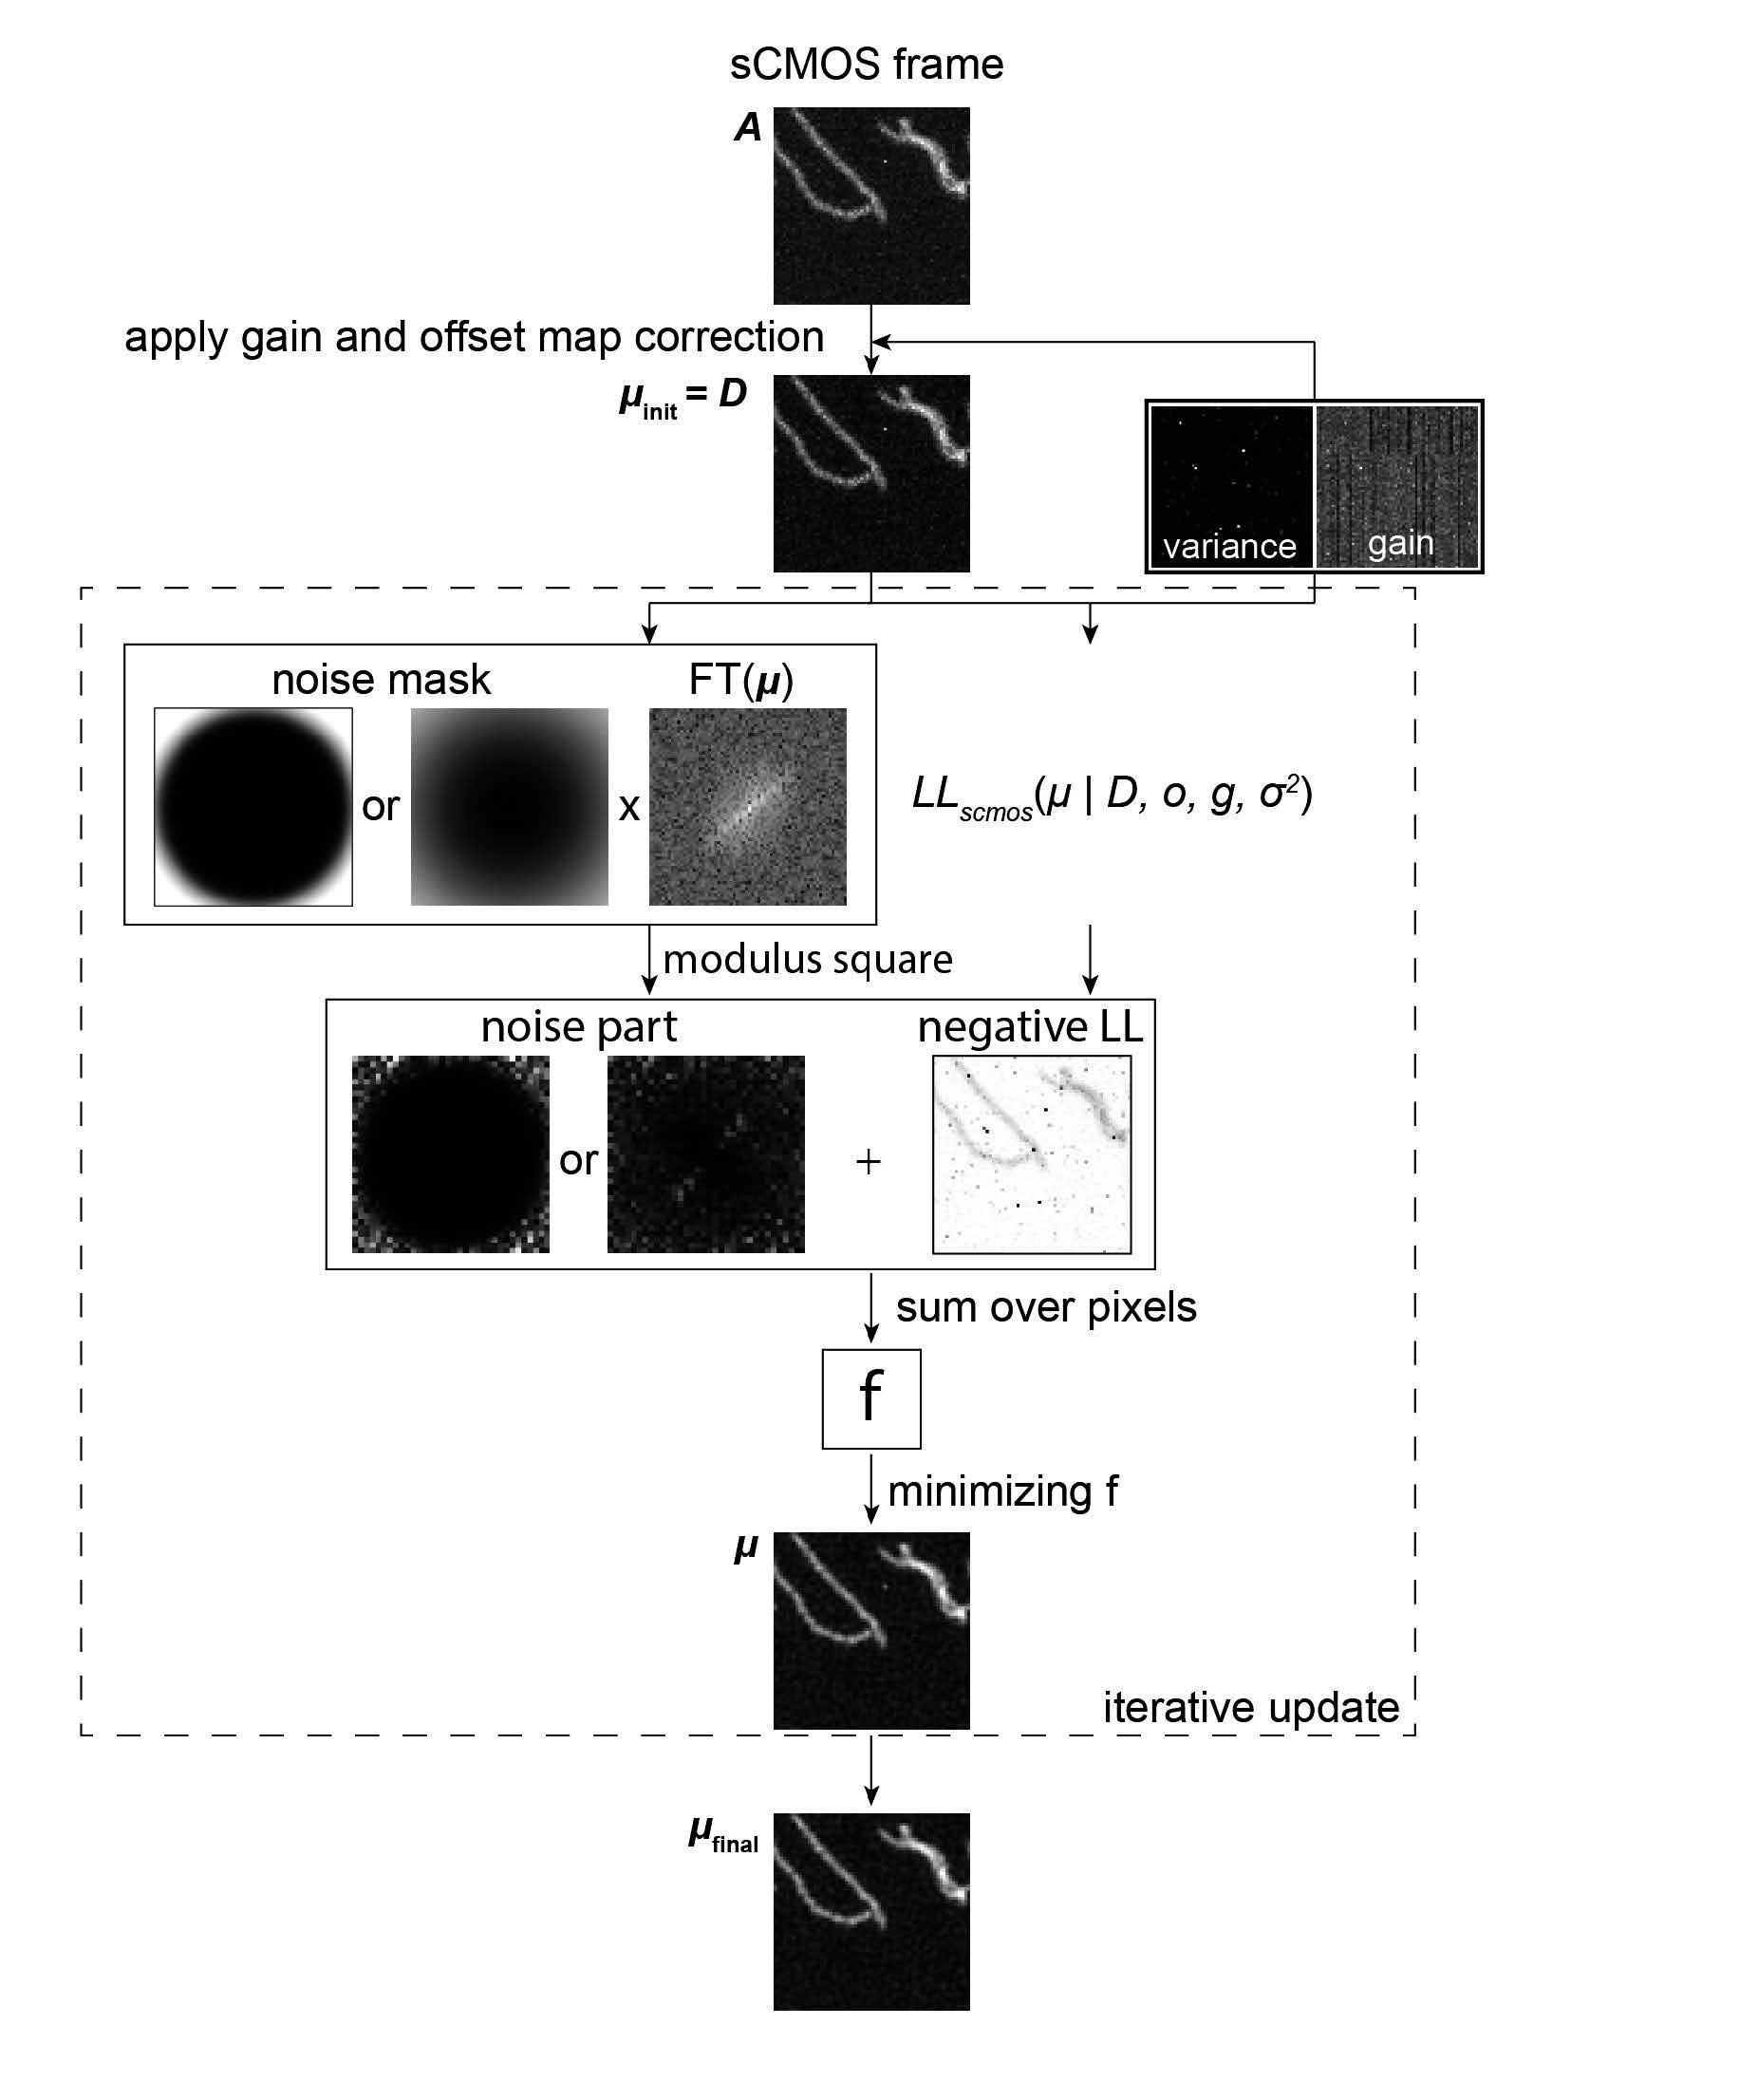
\includegraphics{nmeth.4379-S1.jpg}
\caption{}
\end{figure}

    \begin{Verbatim}[commandchars=\\\{\}]
{\color{incolor}In [{\color{incolor}1}]:} \PY{c+c1}{\PYZsh{} load data}
        \PY{o}{\PYZpc{}}\PY{k}{matplotlib} inline
        \PY{k+kn}{import} \PY{n+nn}{numpy} \PY{k}{as} \PY{n+nn}{np}
        \PY{k+kn}{import} \PY{n+nn}{matplotlib}\PY{n+nn}{.}\PY{n+nn}{pyplot} \PY{k}{as} \PY{n+nn}{plt}
        \PY{k+kn}{import} \PY{n+nn}{h5py}
        \PY{n}{h5f} \PY{o}{=} \PY{n}{h5py}\PY{o}{.}\PY{n}{File}\PY{p}{(}\PY{l+s+s1}{\PYZsq{}}\PY{l+s+s1}{testing\PYZus{}file/TM0000000\PYZus{}CM0\PYZus{}CHN00.h5}\PY{l+s+s1}{\PYZsq{}}\PY{p}{,} \PY{l+s+s1}{\PYZsq{}}\PY{l+s+s1}{r}\PY{l+s+s1}{\PYZsq{}}\PY{p}{)}
        \PY{n}{imgStack} \PY{o}{=} \PY{n}{h5f}\PY{p}{[}\PY{l+s+s1}{\PYZsq{}}\PY{l+s+s1}{default}\PY{l+s+s1}{\PYZsq{}}\PY{p}{]} \PY{c+c1}{\PYZsh{} z, x, y}
        \PY{n}{plt}\PY{o}{.}\PY{n}{imshow}\PY{p}{(}\PY{n}{imgStack}\PY{p}{[}\PY{l+m+mi}{0}\PY{p}{]}\PY{p}{,} \PY{n}{cmap}\PY{o}{=}\PY{l+s+s1}{\PYZsq{}}\PY{l+s+s1}{gray}\PY{l+s+s1}{\PYZsq{}}\PY{p}{)}
        \PY{n}{exImg} \PY{o}{=} \PY{n}{imgStack}\PY{p}{[}\PY{l+m+mi}{0}\PY{p}{]}
\end{Verbatim}


    \begin{Verbatim}[commandchars=\\\{\}]
/Users/dalin/anaconda3/lib/python3.6/site-packages/h5py/\_\_init\_\_.py:36: FutureWarning: Conversion of the second argument of issubdtype from `float` to `np.floating` is deprecated. In future, it will be treated as `np.float64 == np.dtype(float).type`.
  from .\_conv import register\_converters as \_register\_converters

    \end{Verbatim}

    \begin{center}
    \adjustimage{max size={0.9\linewidth}{0.9\paperheight}}{output_3_1.png}
    \end{center}
    { \hspace*{\fill} \\}
    
    \begin{Verbatim}[commandchars=\\\{\}]
{\color{incolor}In [{\color{incolor}2}]:} \PY{n}{M} \PY{o}{=} \PY{l+m+mi}{32} \PY{c+c1}{\PYZsh{} size of segmented image}
\end{Verbatim}


    \begin{Verbatim}[commandchars=\\\{\}]
{\color{incolor}In [{\color{incolor}3}]:} \PY{c+c1}{\PYZsh{} assuming }
        \PY{n}{imgsz} \PY{o}{=} \PY{n}{exImg}\PY{o}{.}\PY{n}{shape}\PY{p}{[}\PY{l+m+mi}{0}\PY{p}{]}\PY{c+c1}{\PYZsh{} image size}
        \PY{k}{assert} \PY{n}{exImg}\PY{o}{.}\PY{n}{shape}\PY{p}{[}\PY{l+m+mi}{0}\PY{p}{]} \PY{o}{==} \PY{n}{exImg}\PY{o}{.}\PY{n}{shape}\PY{p}{[}\PY{l+m+mi}{1}\PY{p}{]}\PY{p}{,} \PY{l+s+s1}{\PYZsq{}}\PY{l+s+s1}{Please crop the image to have the same pixels on x and y}\PY{l+s+s1}{\PYZsq{}}
        \PY{c+c1}{\PYZsh{} the number (imgsz/M)\PYZca{}2 small square patches will be processed in parallel}
\end{Verbatim}


    \section{Characterization of sCMOS
camera}\label{characterization-of-scmos-camera}

\subsection{Offset and variance of sCMOS
camera}\label{offset-and-variance-of-scmos-camera}

Offset values describe a constant level of ADUs (analog-to-digital unit)
pre-engineered into the readout process in order to prevent negative
ADUs caused by the readout noise. Both are estimated by performing
temporally across M dark frames, e.g. \(N = 60,000\). For pixel i

offset: \(o_i = \frac{1}{N}\sum_{n=1}^{N}s_i^n\)

variance: \(v_i = \frac{1}{N}\sum_{n=1}^{N}(s_i^n)^2-o_i^2\)

\subsection{Gain of sCMOS camera}\label{gain-of-scmos-camera}

To determine the gain value for each pixel the authors illuminated the
camera with quasi-uniform stationary intensity patterns and recorded a
series of image sequences (20,000 images in each sequence) at different
average intensity levels ranging from \textasciitilde{}20 to 200 photons
per pixel (totally \(K\) levels). \textbf{This is shot noise and
estimated using Gaussian distribution which approximates the Poisson
distribution}

\(\hat{g_i} = \arg \min \sum_{k=1}^K((v_i^k-v_i)-g_i(<D_i^k>-o_i))^2\)

where \(<D_i^k>\) is mean ADU of all frames at level \(k\), \(v_i^k\) is
the variance.

Let \(A_i\) is a vector \(\{(v_i^1 - v_i), \cdots, (v_i^K - v_i)\}\),
and \(B_i\) is a vector \(\{(<D_i^1> - o_i), \cdots, (<D_i^K> - o_i)\}\)
and \(\hat{g_i} = (B_i B_i^T)^{-1}B_i A_i\).

    \begin{Verbatim}[commandchars=\\\{\}]
{\color{incolor}In [{\color{incolor}4}]:} \PY{c+c1}{\PYZsh{} get offset matrix and variance matrix}
        \PY{c+c1}{\PYZsh{} from glob import glob}
        \PY{c+c1}{\PYZsh{} offset = []}
        \PY{c+c1}{\PYZsh{} var = []}
        \PY{c+c1}{\PYZsh{} for fname in glob(\PYZsq{}/Volumes/ahrenslab/davis/shared/for\PYZus{}ziqiang/blank\PYZus{}frame\PYZus{}mean\PYZus{}variance/t\PYZus{}*.npy\PYZsq{}):}
        \PY{c+c1}{\PYZsh{}     print(\PYZsq{}loading file:\PYZsq{} + fname)}
        \PY{c+c1}{\PYZsh{}     s\PYZus{} = np.load(fname)}
        \PY{c+c1}{\PYZsh{}     offset.append(s\PYZus{}[0])}
        \PY{c+c1}{\PYZsh{}     var.append(s\PYZus{}[1])}
        \PY{c+c1}{\PYZsh{} offset = np.array(offset)}
        \PY{c+c1}{\PYZsh{} var = np.array(var)}
        \PY{c+c1}{\PYZsh{} offset\PYZus{}mat = offset.mean()}
        \PY{c+c1}{\PYZsh{} var\PYZus{}mat = var.mean() + offset.var()}
        \PY{c+c1}{\PYZsh{} gain\PYZus{}mat = np.ones(var\PYZus{}mat.shape)}
\end{Verbatim}


    \begin{Verbatim}[commandchars=\\\{\}]
{\color{incolor}In [{\color{incolor}5}]:} \PY{c+c1}{\PYZsh{} offset = np.load(\PYZsq{}offset\PYZus{}mat.npy\PYZsq{})}
        \PY{c+c1}{\PYZsh{} var = np.load(\PYZsq{}var\PYZus{}mat.npy\PYZsq{})}
        \PY{c+c1}{\PYZsh{} gain = np.load(\PYZsq{}gain\PYZus{}mat.npy\PYZsq{})}
\end{Verbatim}


    \begin{Verbatim}[commandchars=\\\{\}]
{\color{incolor}In [{\color{incolor}6}]:} \PY{c+c1}{\PYZsh{} offset plots, one can easily see some hotspots}
        \PY{c+c1}{\PYZsh{} plt.imshow(offset, cmap=plt.cm.binary)}
\end{Verbatim}


    \begin{Verbatim}[commandchars=\\\{\}]
{\color{incolor}In [{\color{incolor}7}]:} \PY{k+kn}{from} \PY{n+nn}{glob} \PY{k}{import} \PY{n}{glob}
        \PY{n}{offsetMat} \PY{o}{=} \PY{p}{[}\PY{p}{]}\PY{p}{;}
        \PY{n}{varmat} \PY{o}{=} \PY{p}{[}\PY{p}{]}\PY{p}{;}
        \PY{k}{for} \PY{n}{nfile} \PY{o+ow}{in} \PY{n}{glob}\PY{p}{(}\PY{l+s+s1}{\PYZsq{}}\PY{l+s+s1}{camera\PYZus{}statsgain\PYZus{}measure*.npz}\PY{l+s+s1}{\PYZsq{}}\PY{p}{)}\PY{p}{:}
            \PY{n}{data} \PY{o}{=} \PY{n}{np}\PY{o}{.}\PY{n}{load}\PY{p}{(}\PY{n}{nfile}\PY{p}{)}
            \PY{n}{tOff} \PY{o}{=} \PY{n}{data}\PY{p}{[}\PY{l+s+s1}{\PYZsq{}}\PY{l+s+s1}{arr\PYZus{}0}\PY{l+s+s1}{\PYZsq{}}\PY{p}{]}
            \PY{n}{tvar} \PY{o}{=} \PY{n}{data}\PY{p}{[}\PY{l+s+s1}{\PYZsq{}}\PY{l+s+s1}{arr\PYZus{}1}\PY{l+s+s1}{\PYZsq{}}\PY{p}{]}
            \PY{n}{offsetMat}\PY{o}{.}\PY{n}{append}\PY{p}{(}\PY{n}{tOff}\PY{p}{)}
            \PY{n}{varmat}\PY{o}{.}\PY{n}{append}\PY{p}{(}\PY{n}{tvar}\PY{p}{)}
        \PY{n}{offsetMat} \PY{o}{=} \PY{n}{np}\PY{o}{.}\PY{n}{array}\PY{p}{(}\PY{n}{offsetMat}\PY{p}{)}
        \PY{n}{varmat} \PY{o}{=} \PY{n}{np}\PY{o}{.}\PY{n}{array}\PY{p}{(}\PY{n}{varmat}\PY{p}{)}
        \PY{n}{gainMatShape} \PY{o}{=} \PY{p}{(}\PY{n}{varmat}\PY{o}{.}\PY{n}{shape}\PY{p}{[}\PY{l+m+mi}{1}\PY{p}{]}\PY{p}{,} \PY{n}{varmat}\PY{o}{.}\PY{n}{shape}\PY{p}{[}\PY{l+m+mi}{2}\PY{p}{]}\PY{p}{)}
\end{Verbatim}


    \begin{Verbatim}[commandchars=\\\{\}]
{\color{incolor}In [{\color{incolor}8}]:} \PY{c+c1}{\PYZsh{} \PYZsh{} sanity check if pure background is the same as 0mW}
        \PY{c+c1}{\PYZsh{} np.abs(offsetMat[0]\PYZhy{}offset).mean()}
        \PY{c+c1}{\PYZsh{} np.abs(varmat[0]\PYZhy{}var).mean()}
\end{Verbatim}


    \begin{Verbatim}[commandchars=\\\{\}]
{\color{incolor}In [{\color{incolor}9}]:} \PY{c+c1}{\PYZsh{} image to vector}
        \PY{n}{offsetVec} \PY{o}{=} \PY{n}{offsetMat}\PY{o}{.}\PY{n}{reshape}\PY{p}{(}\PY{n}{offsetMat}\PY{o}{.}\PY{n}{shape}\PY{p}{[}\PY{l+m+mi}{0}\PY{p}{]}\PY{p}{,} \PY{o}{\PYZhy{}}\PY{l+m+mi}{1}\PY{p}{)}
        \PY{n}{varVec} \PY{o}{=} \PY{n}{varmat}\PY{o}{.}\PY{n}{reshape}\PY{p}{(}\PY{n}{varmat}\PY{o}{.}\PY{n}{shape}\PY{p}{[}\PY{l+m+mi}{0}\PY{p}{]}\PY{p}{,} \PY{o}{\PYZhy{}}\PY{l+m+mi}{1}\PY{p}{)}
        \PY{c+c1}{\PYZsh{} remove 0mW (background)}
        \PY{n}{offsetVec} \PY{o}{=} \PY{n}{offsetVec} \PY{o}{\PYZhy{}} \PY{n}{offsetVec}\PY{p}{[}\PY{l+m+mi}{0}\PY{p}{]}
        \PY{n}{varVec} \PY{o}{=} \PY{n}{varVec} \PY{o}{\PYZhy{}} \PY{n}{varVec}\PY{p}{[}\PY{l+m+mi}{0}\PY{p}{]}
        \PY{c+c1}{\PYZsh{} remove 0mW}
        \PY{n}{offsetVec} \PY{o}{=} \PY{n}{offsetVec}\PY{p}{[}\PY{l+m+mi}{1}\PY{p}{:}\PY{p}{]}
        \PY{n}{varVec} \PY{o}{=} \PY{n}{varVec}\PY{p}{[}\PY{l+m+mi}{1}\PY{p}{:}\PY{p}{]}
\end{Verbatim}


    \begin{Verbatim}[commandchars=\\\{\}]
{\color{incolor}In [{\color{incolor}10}]:} \PY{n}{gainVec} \PY{o}{=} \PY{n}{np}\PY{o}{.}\PY{n}{zeros}\PY{p}{(}\PY{n}{offsetVec}\PY{o}{.}\PY{n}{shape}\PY{p}{[}\PY{l+m+mi}{1}\PY{p}{]}\PY{p}{)}
         \PY{k}{for} \PY{n}{n} \PY{o+ow}{in} \PY{n+nb}{range}\PY{p}{(}\PY{n}{offsetVec}\PY{o}{.}\PY{n}{shape}\PY{p}{[}\PY{l+m+mi}{1}\PY{p}{]}\PY{p}{)}\PY{p}{:}
             \PY{n}{noffset} \PY{o}{=} \PY{n}{offsetVec}\PY{p}{[}\PY{p}{:}\PY{p}{,} \PY{n}{n}\PY{p}{]}
             \PY{n}{nvar} \PY{o}{=} \PY{n}{varVec}\PY{p}{[}\PY{p}{:}\PY{p}{,} \PY{n}{n}\PY{p}{]}
             \PY{n}{gainVec}\PY{p}{[}\PY{n}{n}\PY{p}{]} \PY{o}{=} \PY{n}{np}\PY{o}{.}\PY{n}{inner}\PY{p}{(}\PY{n}{noffset}\PY{p}{,} \PY{n}{nvar}\PY{p}{)}\PY{o}{/} \PY{n}{np}\PY{o}{.}\PY{n}{inner}\PY{p}{(}\PY{n}{noffset}\PY{p}{,} \PY{n}{noffset}\PY{p}{)}
         
         \PY{n}{offset} \PY{o}{=} \PY{n}{offsetMat}\PY{p}{[}\PY{l+m+mi}{0}\PY{p}{]}
         \PY{n}{var} \PY{o}{=} \PY{n}{varmat}\PY{p}{[}\PY{l+m+mi}{0}\PY{p}{]}
         \PY{n}{gain} \PY{o}{=} \PY{n}{np}\PY{o}{.}\PY{n}{array}\PY{p}{(}\PY{n}{gainVec}\PY{p}{)}\PY{o}{.}\PY{n}{reshape}\PY{p}{(}\PY{n}{gainMatShape}\PY{p}{)}
\end{Verbatim}


    \begin{Verbatim}[commandchars=\\\{\}]
{\color{incolor}In [{\color{incolor}11}]:} \PY{n}{n}\PY{p}{,} \PY{n}{bins}\PY{p}{,} \PY{n}{patches} \PY{o}{=} \PY{n}{plt}\PY{o}{.}\PY{n}{hist}\PY{p}{(}\PY{n}{gainVec}\PY{p}{,} \PY{n}{bins}\PY{o}{=}\PY{l+m+mi}{1000}\PY{p}{,} \PY{n}{density}\PY{o}{=}\PY{k+kc}{True}\PY{p}{,} \PY{n}{facecolor}\PY{o}{=}\PY{l+s+s1}{\PYZsq{}}\PY{l+s+s1}{g}\PY{l+s+s1}{\PYZsq{}}\PY{p}{,} \PY{n}{alpha}\PY{o}{=}\PY{l+m+mf}{0.75}\PY{p}{)}
         \PY{n}{plt}\PY{o}{.}\PY{n}{axis}\PY{p}{(}\PY{p}{[}\PY{l+m+mi}{0}\PY{p}{,} \PY{l+m+mi}{5}\PY{p}{,} \PY{l+m+mi}{0}\PY{p}{,} \PY{l+m+mi}{4}\PY{p}{]}\PY{p}{)}
         \PY{n}{plt}\PY{o}{.}\PY{n}{grid}\PY{p}{(}\PY{k+kc}{True}\PY{p}{)}
         \PY{n}{plt}\PY{o}{.}\PY{n}{show}\PY{p}{(}\PY{p}{)}
\end{Verbatim}


    \begin{center}
    \adjustimage{max size={0.9\linewidth}{0.9\paperheight}}{output_14_0.png}
    \end{center}
    { \hspace*{\fill} \\}
    
    \begin{Verbatim}[commandchars=\\\{\}]
{\color{incolor}In [{\color{incolor}12}]:} \PY{n}{n\PYZus{}pixel} \PY{o}{=} \PY{l+m+mi}{500} \PY{c+c1}{\PYZsh{}np.where(gainVec\PYZlt{}0)[0][0]}
         \PY{n}{x} \PY{o}{=} \PY{n}{np}\PY{o}{.}\PY{n}{array}\PY{p}{(}\PY{p}{[}\PY{l+m+mi}{0}\PY{p}{,} \PY{n}{offsetVec}\PY{p}{[}\PY{p}{:}\PY{p}{,} \PY{n}{n\PYZus{}pixel}\PY{p}{]}\PY{o}{.}\PY{n}{max}\PY{p}{(}\PY{p}{)}\PY{p}{]}\PY{p}{)}
         \PY{n}{y} \PY{o}{=} \PY{n}{x} \PY{o}{*} \PY{n}{gainVec}\PY{p}{[}\PY{n}{n\PYZus{}pixel}\PY{p}{]}
         \PY{n}{plt}\PY{o}{.}\PY{n}{scatter}\PY{p}{(}\PY{n}{offsetVec}\PY{p}{[}\PY{p}{:}\PY{p}{,} \PY{n}{n\PYZus{}pixel}\PY{p}{]}\PY{p}{,} \PY{n}{varVec}\PY{p}{[}\PY{p}{:}\PY{p}{,} \PY{n}{n\PYZus{}pixel}\PY{p}{]}\PY{p}{)}
         \PY{n}{plt}\PY{o}{.}\PY{n}{plot}\PY{p}{(}\PY{n}{x}\PY{p}{,} \PY{n}{y}\PY{p}{,} \PY{l+s+s1}{\PYZsq{}}\PY{l+s+s1}{\PYZhy{}r}\PY{l+s+s1}{\PYZsq{}}\PY{p}{)}
         \PY{n}{plt}\PY{o}{.}\PY{n}{xlabel}\PY{p}{(}\PY{l+s+sa}{r}\PY{l+s+s1}{\PYZsq{}}\PY{l+s+s1}{\PYZdl{}}\PY{l+s+s1}{\PYZbs{}}\PY{l+s+s1}{Delta\PYZdl{} offset}\PY{l+s+s1}{\PYZsq{}}\PY{p}{)}
         \PY{n}{plt}\PY{o}{.}\PY{n}{ylabel}\PY{p}{(}\PY{l+s+sa}{r}\PY{l+s+s1}{\PYZsq{}}\PY{l+s+s1}{\PYZdl{}}\PY{l+s+s1}{\PYZbs{}}\PY{l+s+s1}{Delta\PYZdl{} variance}\PY{l+s+s1}{\PYZsq{}}\PY{p}{)}
         \PY{n}{plt}\PY{o}{.}\PY{n}{title}\PY{p}{(}\PY{l+s+s1}{\PYZsq{}}\PY{l+s+s1}{Pixel index }\PY{l+s+si}{\PYZpc{}s}\PY{l+s+s1}{\PYZsq{}}\PY{o}{\PYZpc{}}\PY{p}{(}\PY{n}{n\PYZus{}pixel}\PY{p}{)}\PY{p}{)}
         \PY{n}{plt}\PY{o}{.}\PY{n}{axis}\PY{p}{(}\PY{p}{[}\PY{l+m+mi}{0}\PY{p}{,} \PY{n}{x}\PY{o}{.}\PY{n}{max}\PY{p}{(}\PY{p}{)}\PY{o}{+}\PY{l+m+mi}{1}\PY{p}{,} \PY{l+m+mi}{0}\PY{p}{,} \PY{n}{y}\PY{o}{.}\PY{n}{max}\PY{p}{(}\PY{p}{)}\PY{o}{+}\PY{l+m+mi}{1}\PY{p}{]}\PY{p}{)}
\end{Verbatim}


\begin{Verbatim}[commandchars=\\\{\}]
{\color{outcolor}Out[{\color{outcolor}12}]:} [0, 65.42812000000012, 0, 157.39119689706266]
\end{Verbatim}
            
    \begin{center}
    \adjustimage{max size={0.9\linewidth}{0.9\paperheight}}{output_15_1.png}
    \end{center}
    { \hspace*{\fill} \\}
    
    \section{OTF}\label{otf}

A diffraction limited imaging system has a cutoff frequency above which
the higher frequency signal cannot be collected. The cutoff frequency is
defined by the numerical aperture (NA), and the detection wavelength
(\(\lambda\)), of the imaging system. The athors used this cutoff
frequency to extract the noise part of the image. Aberrations in the
microscope system might decrease the cutoff frequency which makes the
use of theoretical cutoff a conservative approach. In the 2D Fourier
transform of a microscopy image, the signal from the diffraction limited
system is only contained in a circular region defined by the optical
transfer function (OTF) of the imaging system. The OTF is the
autocorrelation of the pupil function of the imaging system. For an
ideal imaging system, the pupil radius is \(\frac{NA}{\lambda}\), and
the OTF radius is therefore two times of this quantity,
\(2\frac{NA}{\lambda}\).

noise contribution in 2D transformed image \(U\) is calculated as

\(\sigma = \sum_{k_x, k_y}|U(k_x, k_y)M(k_x, k_y)|\)

\subsection{Parameters}\label{parameters}

\begin{itemize}
\tightlist
\item
  NA: numerical aperture of the objective
\item
  \(\lambda\): emission wavelength (micro-meter, um)
\item
  \(\Delta x = \Delta y\): pixel size (um) of the image in two
  dimensions, these are used to compute the 2D transform of the image,
  u(x, y) with L by L pixels as
  \(U(k_x, k_y) = \frac{1}{L}\sum_x\sum_y u(x, y) \exp(-i2\pi k_x x)\exp(-i2\pi k_y y)\)
\end{itemize}

\subsection{OTF mask}\label{otf-mask}

The OTF mask is implemented using a raised cosine filter defined by two
parameters \(\beta\) and \(T\).

\(M(k_x, k_y) = 1\) if \(k_r = \sqrt{k_x^2 + k_y^2}>\frac{1+\beta}{2T}\)

\(M(k_x, k_y) = 0\) if \(k_r < \frac{1-\beta}{2T}\)

\(M(k_x, k_y) = \frac{1}{2} + \frac{1}{2}\cos[\frac{\pi T}{\beta}(k_r - \frac{1-\beta}{2T})]\)
if otherwise

One can use one of the follow OTF masks: 1. OTF weighted mask
(\textbf{default}; better peformance in denoising, but signal would be
decreased, comparin to noise-only mask) \(\beta = 1\),
\(T = \frac{\lambda}{4NA*1.4}\), 2. Noise-only mask: \(\beta = 0.2\),
\(T = \frac{(1-\beta)\lambda}{4NA}\), 3. An adjustable version of
weighted mask (using additional parameters like \(w\) and \(h\)):
\(\beta = \pi/2*\frac{k_{max}/w_0-1}{\arccos(1-2*h)+\pi/2*(k_{max}/w_0-1)}\),
\(T = \frac{1-\beta}{2w_0}\), \(w_0 = w*\frac{NA}{\lambda}\)

    \begin{Verbatim}[commandchars=\\\{\}]
{\color{incolor}In [{\color{incolor}13}]:} \PY{n}{Pixelsize} \PY{o}{=} \PY{l+m+mf}{6.5} \PY{c+c1}{\PYZsh{} pixel size is the property of the camera (make sure this value is correct)}
         \PY{n}{Magnification} \PY{o}{=} \PY{l+m+mi}{16}
         \PY{n}{Pixelsize} \PY{o}{=} \PY{n}{Pixelsize} \PY{o}{/} \PY{n}{Magnification}
         \PY{n}{NA} \PY{o}{=} \PY{l+m+mf}{0.8} \PY{c+c1}{\PYZsh{} numerical aperture of the objective}
         \PY{c+c1}{\PYZsh{} emission should be changed according to the real experiment}
         \PY{n}{Lambda} \PY{o}{=} \PY{l+m+mf}{0.500} \PY{c+c1}{\PYZsh{} emission wavelength}
         \PY{n}{w}\PY{o}{=}\PY{l+m+mi}{1} \PY{c+c1}{\PYZsh{} parameter for adjusted OTF}
         \PY{n}{h}\PY{o}{=}\PY{l+m+mf}{0.7} \PY{c+c1}{\PYZsh{} parameter for adjusted OTF}
\end{Verbatim}


    \begin{Verbatim}[commandchars=\\\{\}]
{\color{incolor}In [{\color{incolor}14}]:} \PY{k+kn}{import} \PY{n+nn}{denoisetools} \PY{k}{as} \PY{n+nn}{ncs}
\end{Verbatim}


    \begin{Verbatim}[commandchars=\\\{\}]
{\color{incolor}In [{\color{incolor}15}]:} \PY{c+c1}{\PYZsh{} \PYZsh{}OTF filter}
         \PY{c+c1}{\PYZsh{} OTFfilter = ncs.genfilter(M,Pixelsize,NA,Lambda,Type=\PYZsq{}OTFweighted\PYZsq{},w=1,h=0.7)}
         \PY{c+c1}{\PYZsh{} plt.imshow(OTFfilter, cmap = plt.cm.gray)}
         \PY{c+c1}{\PYZsh{} plt.colorbar()}
\end{Verbatim}


    \begin{Verbatim}[commandchars=\\\{\}]
{\color{incolor}In [{\color{incolor}16}]:} \PY{c+c1}{\PYZsh{} plt.scatter(offset.reshape(\PYZhy{}1), np.sqrt(var.reshape(\PYZhy{}1)))}
         \PY{c+c1}{\PYZsh{} plt.xlabel(\PYZdq{}Offset\PYZdq{})}
         \PY{c+c1}{\PYZsh{} plt.ylabel(\PYZdq{}Std.\PYZdq{})}
\end{Verbatim}


    \begin{Verbatim}[commandchars=\\\{\}]
{\color{incolor}In [{\color{incolor}17}]:} \PY{c+c1}{\PYZsh{} preprocessing of image}
         \PY{n}{imgD} \PY{o}{=} \PY{p}{(}\PY{n}{imgStack}\PY{p}{[}\PY{l+m+mi}{0}\PY{p}{]}\PY{o}{\PYZhy{}}\PY{n}{offset}\PY{p}{)}\PY{o}{/}\PY{n}{gain}
         \PY{n}{imgD}\PY{p}{[}\PY{n}{gain}\PY{o}{\PYZlt{}}\PY{l+m+mi}{0}\PY{p}{]} \PY{o}{=} \PY{l+m+mf}{1e\PYZhy{}6}
         \PY{n}{imgD}\PY{p}{[}\PY{n}{imgD}\PY{o}{\PYZlt{}}\PY{o}{=}\PY{l+m+mi}{0}\PY{p}{]} \PY{o}{=} \PY{l+m+mf}{1e\PYZhy{}6}
\end{Verbatim}


    \begin{Verbatim}[commandchars=\\\{\}]
{\color{incolor}In [{\color{incolor}18}]:} \PY{c+c1}{\PYZsh{} crop image}
         \PY{n}{imgD\PYZus{}} \PY{o}{=} \PY{n}{imgD}\PY{p}{[}\PY{l+m+mi}{512}\PY{p}{:}\PY{l+m+mi}{1024}\PY{p}{,} \PY{l+m+mi}{512}\PY{p}{:}\PY{l+m+mi}{1024}\PY{p}{]}
         \PY{n}{gain\PYZus{}} \PY{o}{=} \PY{n}{gain}\PY{p}{[}\PY{l+m+mi}{512}\PY{p}{:}\PY{l+m+mi}{1024}\PY{p}{,} \PY{l+m+mi}{512}\PY{p}{:}\PY{l+m+mi}{1024}\PY{p}{]}
         \PY{n}{gain\PYZus{}}\PY{p}{[}\PY{n}{gain\PYZus{}} \PY{o}{\PYZlt{}} \PY{l+m+mi}{0}\PY{p}{]} \PY{o}{=} \PY{l+m+mf}{1e\PYZhy{}6}
         \PY{n}{var\PYZus{}} \PY{o}{=} \PY{n}{var}\PY{p}{[}\PY{l+m+mi}{512}\PY{p}{:}\PY{l+m+mi}{1024}\PY{p}{,} \PY{l+m+mi}{512}\PY{p}{:}\PY{l+m+mi}{1024}\PY{p}{]}
         
         \PY{c+c1}{\PYZsh{} imgD\PYZus{} = imgD}
         \PY{c+c1}{\PYZsh{} imgD\PYZus{}[imgD\PYZus{} \PYZlt{} 0] = 1e\PYZhy{}6}
         \PY{c+c1}{\PYZsh{} gain\PYZus{} = gain}
         \PY{c+c1}{\PYZsh{} var\PYZus{} = var}
\end{Verbatim}


    \begin{Verbatim}[commandchars=\\\{\}]
{\color{incolor}In [{\color{incolor}42}]:} \PY{n}{alpha} \PY{o}{=} \PY{l+m+mf}{0.1} \PY{c+c1}{\PYZsh{} weight factor of noise correction contribution vs LLS (simplified negative log likelihood function)}
         \PY{n}{iterationN} \PY{o}{=} \PY{l+m+mi}{15} \PY{c+c1}{\PYZsh{} number of iterations}
\end{Verbatim}


    \begin{Verbatim}[commandchars=\\\{\}]
{\color{incolor}In [{\color{incolor}43}]:} \PY{c+c1}{\PYZsh{} \PYZsh{} optical transfer function filter is defined using filter type (default is OTFweighted), w and h}
         \PY{n}{out} \PY{o}{=} \PY{n}{ncs}\PY{o}{.}\PY{n}{reducenoise}\PY{p}{(}\PY{n}{M}\PY{p}{,} \PY{n}{imgD\PYZus{}}\PY{p}{,}\PY{n}{var\PYZus{}}\PY{p}{,}\PY{n}{gain\PYZus{}}\PY{p}{,}\PY{n}{Pixelsize}\PY{p}{,}\PY{n}{NA}\PY{p}{,}\PY{n}{Lambda}\PY{p}{,}\PY{n}{alpha}\PY{p}{,}\PY{n}{iterationN}\PY{p}{)}
\end{Verbatim}


    \begin{Verbatim}[commandchars=\\\{\}]
Elapsed time for noise reduction: 119.20078897476196

    \end{Verbatim}

    \begin{Verbatim}[commandchars=\\\{\}]
{\color{incolor}In [{\color{incolor}44}]:} \PY{n}{out}\PY{p}{[}\PY{n}{gain\PYZus{}}\PY{o}{\PYZlt{}}\PY{l+m+mi}{0}\PY{p}{]} \PY{o}{=} \PY{l+m+mf}{1e\PYZhy{}6}
         \PY{n}{out\PYZus{}} \PY{o}{=} \PY{n}{out}
         \PY{n}{out\PYZus{}}\PY{p}{[}\PY{n}{gain\PYZus{}}\PY{o}{\PYZlt{}}\PY{l+m+mf}{0.5}\PY{p}{]} \PY{o}{=} \PY{l+m+mf}{1e\PYZhy{}6}
         \PY{n}{imgD\PYZus{}}\PY{p}{[}\PY{n}{gain\PYZus{}}\PY{o}{\PYZlt{}}\PY{l+m+mf}{0.5}\PY{p}{]} \PY{o}{=} \PY{l+m+mf}{1e\PYZhy{}6}
\end{Verbatim}


    \begin{Verbatim}[commandchars=\\\{\}]
{\color{incolor}In [{\color{incolor}45}]:} \PY{n}{f}\PY{p}{,} \PY{p}{(}\PY{n}{ax1}\PY{p}{,} \PY{n}{ax2}\PY{p}{,} \PY{n}{ax3}\PY{p}{)} \PY{o}{=} \PY{n}{plt}\PY{o}{.}\PY{n}{subplots}\PY{p}{(}\PY{l+m+mi}{1}\PY{p}{,} \PY{l+m+mi}{3}\PY{p}{)}
         \PY{n}{ax1}\PY{o}{.}\PY{n}{imshow}\PY{p}{(}\PY{n}{imgStack}\PY{p}{[}\PY{l+m+mi}{0}\PY{p}{]}\PY{p}{[}\PY{l+m+mi}{512}\PY{p}{:}\PY{l+m+mi}{1024}\PY{p}{,} \PY{l+m+mi}{512}\PY{p}{:}\PY{l+m+mi}{1024}\PY{p}{]}\PY{p}{,} \PY{n}{cmap}\PY{o}{=}\PY{l+s+s1}{\PYZsq{}}\PY{l+s+s1}{gray}\PY{l+s+s1}{\PYZsq{}}\PY{p}{)}
         \PY{c+c1}{\PYZsh{} ax1.imshow(imgStack[0], cmap=\PYZsq{}gray\PYZsq{})}
         \PY{n}{ax1}\PY{o}{.}\PY{n}{set\PYZus{}title}\PY{p}{(}\PY{l+s+s1}{\PYZsq{}}\PY{l+s+s1}{Raw image}\PY{l+s+s1}{\PYZsq{}}\PY{p}{)}
         \PY{n}{ax1}\PY{o}{.}\PY{n}{axis}\PY{p}{(}\PY{l+s+s1}{\PYZsq{}}\PY{l+s+s1}{off}\PY{l+s+s1}{\PYZsq{}}\PY{p}{)}
         \PY{n}{ax2}\PY{o}{.}\PY{n}{imshow}\PY{p}{(}\PY{n}{imgD\PYZus{}}\PY{p}{,} \PY{n}{cmap}\PY{o}{=}\PY{l+s+s1}{\PYZsq{}}\PY{l+s+s1}{gray}\PY{l+s+s1}{\PYZsq{}}\PY{p}{)}
         \PY{n}{ax2}\PY{o}{.}\PY{n}{set\PYZus{}title}\PY{p}{(}\PY{l+s+s1}{\PYZsq{}}\PY{l+s+s1}{Preprocessed}\PY{l+s+s1}{\PYZsq{}}\PY{p}{)}
         \PY{n}{ax2}\PY{o}{.}\PY{n}{axis}\PY{p}{(}\PY{l+s+s1}{\PYZsq{}}\PY{l+s+s1}{off}\PY{l+s+s1}{\PYZsq{}}\PY{p}{)}
         \PY{n}{ax3}\PY{o}{.}\PY{n}{imshow}\PY{p}{(}\PY{n}{out\PYZus{}}\PY{p}{,} \PY{n}{cmap}\PY{o}{=}\PY{l+s+s1}{\PYZsq{}}\PY{l+s+s1}{gray}\PY{l+s+s1}{\PYZsq{}}\PY{p}{)}
         \PY{n}{ax3}\PY{o}{.}\PY{n}{set\PYZus{}title}\PY{p}{(}\PY{l+s+s1}{\PYZsq{}}\PY{l+s+s1}{Denoised image}\PY{l+s+s1}{\PYZsq{}}\PY{p}{)}
         \PY{n}{ax3}\PY{o}{.}\PY{n}{axis}\PY{p}{(}\PY{l+s+s1}{\PYZsq{}}\PY{l+s+s1}{off}\PY{l+s+s1}{\PYZsq{}}\PY{p}{)}
         \PY{n}{f}\PY{o}{.}\PY{n}{savefig}\PY{p}{(}\PY{l+s+s1}{\PYZsq{}}\PY{l+s+s1}{comparison.png}\PY{l+s+s1}{\PYZsq{}}\PY{p}{,} \PY{n}{dpi}\PY{o}{=}\PY{l+m+mi}{1000}\PY{p}{)}
         \PY{n}{plt}\PY{o}{.}\PY{n}{show}\PY{p}{(}\PY{p}{)}
\end{Verbatim}


    \begin{center}
    \adjustimage{max size={0.9\linewidth}{0.9\paperheight}}{output_26_0.png}
    \end{center}
    { \hspace*{\fill} \\}
    
    \begin{Verbatim}[commandchars=\\\{\}]
{\color{incolor}In [{\color{incolor}55}]:} \PY{k}{for} \PY{n}{alpha} \PY{o+ow}{in} \PY{p}{[}\PY{l+m+mi}{0}\PY{p}{,} \PY{l+m+mf}{0.1}\PY{p}{,} \PY{l+m+mf}{0.9}\PY{p}{,} \PY{l+m+mi}{9}\PY{p}{]}\PY{p}{:}
             \PY{n}{out} \PY{o}{=} \PY{n}{ncs}\PY{o}{.}\PY{n}{reducenoise}\PY{p}{(}\PY{n}{M}\PY{p}{,} \PY{n}{imgD\PYZus{}}\PY{p}{,}\PY{n}{var\PYZus{}}\PY{p}{,}\PY{n}{gain\PYZus{}}\PY{p}{,}\PY{n}{Pixelsize}\PY{p}{,}\PY{n}{NA}\PY{p}{,}\PY{n}{Lambda}\PY{p}{,}\PY{n}{alpha}\PY{p}{,}\PY{n}{iterationN}\PY{p}{)}
             \PY{n}{out}\PY{p}{[}\PY{n}{gain\PYZus{}}\PY{o}{\PYZlt{}}\PY{l+m+mi}{0}\PY{p}{]} \PY{o}{=} \PY{l+m+mf}{1e\PYZhy{}6}
             \PY{n}{out\PYZus{}} \PY{o}{=} \PY{n}{out}
             \PY{n}{out\PYZus{}}\PY{p}{[}\PY{n}{gain\PYZus{}}\PY{o}{\PYZlt{}}\PY{l+m+mf}{0.5}\PY{p}{]} \PY{o}{=} \PY{l+m+mf}{1e\PYZhy{}6}
             \PY{n}{plt}\PY{o}{.}\PY{n}{imshow}\PY{p}{(}\PY{n}{out\PYZus{}}\PY{p}{,} \PY{n}{cmap}\PY{o}{=}\PY{l+s+s1}{\PYZsq{}}\PY{l+s+s1}{gray}\PY{l+s+s1}{\PYZsq{}}\PY{p}{)}
             \PY{n}{plt}\PY{o}{.}\PY{n}{title}\PY{p}{(}\PY{l+s+sa}{r}\PY{l+s+s1}{\PYZsq{}}\PY{l+s+s1}{\PYZdl{}}\PY{l+s+s1}{\PYZbs{}}\PY{l+s+s1}{alpha\PYZdl{} = }\PY{l+s+si}{\PYZpc{}0.1f}\PY{l+s+s1}{\PYZsq{}}\PY{o}{\PYZpc{}}\PY{k}{alpha})
             \PY{n}{plt}\PY{o}{.}\PY{n}{show}\PY{p}{(}\PY{p}{)}
             \PY{n}{diff} \PY{o}{=} \PY{n}{np}\PY{o}{.}\PY{n}{abs}\PY{p}{(}\PY{n}{out\PYZus{}} \PY{o}{\PYZhy{}} \PY{n}{imgD\PYZus{}}\PY{p}{)}\PY{o}{/}\PY{n}{imgD\PYZus{}}
             \PY{n+nb}{print}\PY{p}{(}\PY{n}{diff}\PY{o}{.}\PY{n}{max}\PY{p}{(}\PY{p}{)}\PY{p}{)}
\end{Verbatim}


    \begin{Verbatim}[commandchars=\\\{\}]
Elapsed time for noise reduction: 89.48394393920898

    \end{Verbatim}

    \begin{center}
    \adjustimage{max size={0.9\linewidth}{0.9\paperheight}}{output_27_1.png}
    \end{center}
    { \hspace*{\fill} \\}
    
    \begin{Verbatim}[commandchars=\\\{\}]
4.926970136032264e-07
Elapsed time for noise reduction: 175.58020663261414

    \end{Verbatim}

    \begin{center}
    \adjustimage{max size={0.9\linewidth}{0.9\paperheight}}{output_27_3.png}
    \end{center}
    { \hspace*{\fill} \\}
    
    \begin{Verbatim}[commandchars=\\\{\}]
90013.1695008107
Elapsed time for noise reduction: 160.7814600467682

    \end{Verbatim}

    \begin{center}
    \adjustimage{max size={0.9\linewidth}{0.9\paperheight}}{output_27_5.png}
    \end{center}
    { \hspace*{\fill} \\}
    
    \begin{Verbatim}[commandchars=\\\{\}]
728498.6892470393
Elapsed time for noise reduction: 162.2573459148407

    \end{Verbatim}

    \begin{center}
    \adjustimage{max size={0.9\linewidth}{0.9\paperheight}}{output_27_7.png}
    \end{center}
    { \hspace*{\fill} \\}
    
    \begin{Verbatim}[commandchars=\\\{\}]
5232581.977193492

    \end{Verbatim}

    \subsection{How is the denoised image compared to the one with
preprocessing?}\label{how-is-the-denoised-image-compared-to-the-one-with-preprocessing}

\subsubsection{Preprocessing imaging is defined as
D}\label{preprocessing-imaging-is-defined-as-d}

\(D_i = (I_i - o_i)/\hat{g}_i\)

\subsubsection{Comparison}\label{comparison}

\begin{enumerate}
\def\labelenumi{\arabic{enumi}.}
\item
  compare the accumulated distribution between denoised image vs
  preprocessing image -\/- it has a visual difference at value ranged
  from 10 to 30
\item
  compare the relative change between denoised image vs preprocessing
  image at range from 10 to 30 -\/- relative change is defined as
  \(|D_i - \hat{D}_i|/D_i\), which is quite small
\end{enumerate}

    \begin{Verbatim}[commandchars=\\\{\}]
{\color{incolor}In [{\color{incolor}83}]:} \PY{n}{out\PYZus{}\PYZus{}} \PY{o}{=} \PY{n}{out\PYZus{}}\PY{p}{[}\PY{n}{imgD\PYZus{}} \PY{o}{\PYZgt{}} \PY{l+m+mi}{0}\PY{p}{]}
         \PY{n}{imgD\PYZus{}\PYZus{}} \PY{o}{=} \PY{n}{imgD\PYZus{}}\PY{p}{[}\PY{n}{imgD\PYZus{}} \PY{o}{\PYZgt{}} \PY{l+m+mi}{0}\PY{p}{]}
         \PY{n}{values}\PY{p}{,} \PY{n}{base} \PY{o}{=} \PY{n}{np}\PY{o}{.}\PY{n}{histogram}\PY{p}{(}\PY{n}{out\PYZus{}\PYZus{}}\PY{p}{,} \PY{n}{bins}\PY{o}{=}\PY{l+m+mi}{1000}\PY{p}{)}
         \PY{c+c1}{\PYZsh{}evaluate the cumulative}
         \PY{n}{cumulative} \PY{o}{=} \PY{n}{np}\PY{o}{.}\PY{n}{cumsum}\PY{p}{(}\PY{n}{values}\PY{p}{)}\PY{o}{/}\PY{n+nb}{len}\PY{p}{(}\PY{n}{out\PYZus{}\PYZus{}}\PY{p}{)}
         \PY{c+c1}{\PYZsh{} plot the cumulative function}
         \PY{n}{plt}\PY{o}{.}\PY{n}{plot}\PY{p}{(}\PY{n}{base}\PY{p}{[}\PY{p}{:}\PY{o}{\PYZhy{}}\PY{l+m+mi}{1}\PY{p}{]}\PY{p}{,} \PY{n}{cumulative}\PY{p}{,} \PY{n}{c}\PY{o}{=}\PY{l+s+s1}{\PYZsq{}}\PY{l+s+s1}{blue}\PY{l+s+s1}{\PYZsq{}}\PY{p}{,}\PY{n}{label}\PY{o}{=}\PY{l+s+s1}{\PYZsq{}}\PY{l+s+s1}{denoised}\PY{l+s+s1}{\PYZsq{}}\PY{p}{)}
         \PY{n}{values}\PY{p}{,} \PY{n}{base} \PY{o}{=} \PY{n}{np}\PY{o}{.}\PY{n}{histogram}\PY{p}{(}\PY{n}{imgD\PYZus{}\PYZus{}}\PY{p}{,} \PY{n}{bins}\PY{o}{=}\PY{l+m+mi}{1000}\PY{p}{)}
         \PY{c+c1}{\PYZsh{}evaluate the cumulative}
         \PY{n}{cumulative} \PY{o}{=} \PY{n}{np}\PY{o}{.}\PY{n}{cumsum}\PY{p}{(}\PY{n}{values}\PY{p}{)}\PY{o}{/}\PY{n+nb}{len}\PY{p}{(}\PY{n}{imgD\PYZus{}\PYZus{}}\PY{p}{)}
         \PY{c+c1}{\PYZsh{} plot the cumulative function}
         \PY{n}{plt}\PY{o}{.}\PY{n}{plot}\PY{p}{(}\PY{n}{base}\PY{p}{[}\PY{p}{:}\PY{o}{\PYZhy{}}\PY{l+m+mi}{1}\PY{p}{]}\PY{p}{,} \PY{n}{cumulative}\PY{p}{,} \PY{n}{c}\PY{o}{=}\PY{l+s+s1}{\PYZsq{}}\PY{l+s+s1}{red}\PY{l+s+s1}{\PYZsq{}}\PY{p}{,}\PY{n}{label}\PY{o}{=}\PY{l+s+s1}{\PYZsq{}}\PY{l+s+s1}{preprocessing}\PY{l+s+s1}{\PYZsq{}}\PY{p}{)}
         \PY{n}{plt}\PY{o}{.}\PY{n}{xlabel}\PY{p}{(}\PY{l+s+s1}{\PYZsq{}}\PY{l+s+s1}{corrected pixel value}\PY{l+s+s1}{\PYZsq{}}\PY{p}{)}
         \PY{n}{plt}\PY{o}{.}\PY{n}{ylabel}\PY{p}{(}\PY{l+s+s1}{\PYZsq{}}\PY{l+s+s1}{accumulated frac.}\PY{l+s+s1}{\PYZsq{}}\PY{p}{)}
         \PY{n}{plt}\PY{o}{.}\PY{n}{legend}\PY{p}{(}\PY{p}{)}
         \PY{n}{plt}\PY{o}{.}\PY{n}{show}\PY{p}{(}\PY{p}{)}
\end{Verbatim}


    \begin{center}
    \adjustimage{max size={0.9\linewidth}{0.9\paperheight}}{output_29_0.png}
    \end{center}
    { \hspace*{\fill} \\}
    
    \begin{Verbatim}[commandchars=\\\{\}]
{\color{incolor}In [{\color{incolor}87}]:} \PY{n}{diff\PYZus{}} \PY{o}{=} \PY{n}{diff}\PY{p}{[}\PY{n}{np}\PY{o}{.}\PY{n}{logical\PYZus{}and}\PY{p}{(}\PY{n}{imgD\PYZus{}} \PY{o}{\PYZgt{}} \PY{l+m+mi}{10}\PY{p}{,} \PY{n}{imgD\PYZus{}}\PY{o}{\PYZlt{}}\PY{l+m+mi}{30}\PY{p}{)}\PY{p}{]}
         \PY{n}{\PYZus{}}\PY{p}{,} \PY{n}{\PYZus{}}\PY{p}{,} \PY{n}{\PYZus{}} \PY{o}{=} \PY{n}{plt}\PY{o}{.}\PY{n}{hist}\PY{p}{(}\PY{n}{diff\PYZus{}}\PY{p}{,} \PY{l+m+mi}{1000}\PY{p}{)}
         \PY{n}{plt}\PY{o}{.}\PY{n}{ylabel}\PY{p}{(}\PY{l+s+s1}{\PYZsq{}}\PY{l+s+s1}{counts}\PY{l+s+s1}{\PYZsq{}}\PY{p}{)}
         \PY{n}{plt}\PY{o}{.}\PY{n}{xlabel}\PY{p}{(}\PY{l+s+s1}{\PYZsq{}}\PY{l+s+s1}{relative change}\PY{l+s+s1}{\PYZsq{}}\PY{p}{)}
         \PY{n}{plt}\PY{o}{.}\PY{n}{show}\PY{p}{(}\PY{p}{)}
\end{Verbatim}


    \begin{center}
    \adjustimage{max size={0.9\linewidth}{0.9\paperheight}}{output_30_0.png}
    \end{center}
    { \hspace*{\fill} \\}
    

    % Add a bibliography block to the postdoc
    
    
    
    \end{document}
